\documentclass[conference]{IEEEtran}
\usepackage{url}
\usepackage[utf8]{inputenc}
\usepackage{amsmath,mathtools}
\usepackage[backend=biber,style=ieee]{biblatex}
 %https://tex.stackexchange.com/questions/112576/math-mode-in-tabular-without-having-to-use-everywhere
\usepackage{array}   % for \newcolumntype macro
\usepackage{caption}
\newcolumntype{C}{>{$}c<{$}} % math-mode version of "l" column type

\addbibresource{biblio.bib}
\newcommand{\ro}{$R_0$}

\begin{document}
\title{Modeling the Spread of Measles}

\author{\IEEEauthorblockN{Nima Seyedtalebi,
Joseph Kaninberg,
Seifalla Moustafa
}
\IEEEauthorblockA{Department of Computer Science\\
University of Kentucky\\
Lexington, KY 40506--0633}
}
\maketitle



\begin{abstract} %Joe
In order to ascertain behavioral information related to a particular disease, it is integral that the propagation of said disease can be accurately modeled mathematically. Typically, this is accomplished by using a wealth of historical data related to any given disease. It is often the case that no one model can accurately demonstrate all behaviors of a disease realistically. As such, this paper will motivate and discuss a model specifically designed to simulate the propagation of Measles within an interaction based network. In doing so, the authors hope to provide and demonstrate a model that can be used to exclusively simulate measles behavior with a high degree of accuracy. Our model is a variation of [SEIR] model. We introduce the interaction graph based method in which nodes represent individuals and edges represent interactions.The transition from each state in the [SEIR] to another i.e E to I or I to R is determined by thresholds of each node.
The authors consider a number of terms such as secondary infection rate, infection and incubation periods and the basic reproduction number $R_0$.
By comparing the results of our model to the historical results we found that it works well and can be considered as a reference.
\end{abstract}

\section{Introduction} %Joe
The ability to accurately model the propagation of a disease within a given population is a key component in discerning relevant attributes related to the disease being propagated. The generalization of disease propagation simulation to reality hinges upon the ability to accurately model the phenomena within a simulated setting. Typically, this is accomplished by making use of historical data in order to ascertain unique aspects related to the simulated disease. Using these unique aspects, simulations can be run in order to model the general propagation trends of the disease. In most cases, the quickness of propagation and varying infection rates due to personal contact are important factors. Due to the importance of interaction in disease propagation, interaction modeling is given a reasonable amount of attention. Often, this personal contact factor is simulated in one of two ways. The first is a stochastic method, while the remaining is an interaction network based method. In the stochastic simulation method, spreading occurs in a manner that is purely probability based, so a large number of simulations are needed to produce accurate results. In an interaction graph based method, individuals are modeled as vertices and sufficient interactions as edges. In some cases, hybrid models are produced in which both interaction methods are taken into account and intertwined.\par
The modeling of epidemic spreading within a community is an extremely well researched area in modern scientific inquiry. With the advent of modern vaccinations, certain diseases have all but died out and become of little to no concern to the general populace. Due to the rise of the anti-vaccination sentiment however, many previously dying diseases are beginning to propagate among human populations once more. With this sentiment becoming increasingly prominent, it would be wise to examine historical data relating to these previous deadly diseases. In particular, diseases such as measles have been given a 'second-wind' so to speak. As a result, the need to accurately simulate these diseases in order to help mitigate the potential harm done by these infections has become increasingly important. As such, models used to simulate these diseases need to be developed in order to help minimize the potential risks.\par
For modeling the spread of disease, it is common practice to use a pre-established model that applies to general propagation phenomena. For disease propagation, however, this method can be reasonably unreliable due to the variance in individual disease behaviors. As such, it is often appropriate to develop individual models that can be used to accurately model the behavior and propagation phenomena demonstrated by a single disease. With this in mind, this paper seeks to model the behavior and spreading of measles using a model specifically designed to simulate these aspects of the infection. This paper seeks to demonstrate the accuracy and viability of the proposed model by comparing the results to historical behavioral data related to measles. 

\section{Related Work} %Joe
In general, the modeling and simulation of diseases propagation is often implemented using an already existing model as a base. The most simplistic model that demonstrates propagation capabilities is the Susceptible-Infected (SI) model. In this model, individuals are either unexposed to an infection or infected. Due to the simplicity of the model, it is often a poor means by which to model the propagation of actual diseases. An improvement is made by the SIR model, which adds a recovered compartment that is used to account for individuals that have either survived or perished from the disease. Some models make a distinction between recovery and death, but most rarely differentiate between them. Often, these types of models work well for information diffusion modeling \cite{Tambuscio15} rather than disease propagation modeling. As the primary goal of this paper is the accurate modeling of measles, unfitting models for this topic will be disregarded. Often, models that demonstrate interesting behavior on complex networks behave in a fashion that facilitates better accuracy in modeling disease propagation \cite{Hethcote2000TheMO,Pastor_satorras2014}. An even better approximation model than the SIR model for use in modeling disease propagation is described by Hethcote \cite{Hethcote2000TheMO}. In particular, he presents a Susceptible-Exposed-Infected-Recovered (SEIR) model and a number of variations of the model due to changing disease behavioral phenomena. The SEIR model described by Hethcote has been compared to real world infection data through simulations, demonstrating a reasonable degree of accuracy \cite{Montalan19}. The model forwarded later by this paper is a variation of Hethcote's SEIR model, except that the proposed model does not have a dynamically changing population size similar to the one presented in Hethcote's model \cite{Hethcote2000TheMO}.\par
Many studies have been published examining or analyzing the general propagation of diseases within a specific real-world population \cite{pinkbookMeasles,measlesIncidence,Jasem2012Elsevier,Mcbrein2003,Sugarman2010}. Using these findings, various models have been proposed with the intent of accurately modeling properties of measles described by related studies. Most of these models are reasonably successful, but there are still a number of areas in which improvement is needed. For example, the initial infection rate of measles is rarely considered in most models. It is also often the case that the number of individuals within a compartment- susceptible, exposed, infected, and recovered-are fit to a graph for the model, but an accurate simulation of similar time scaling is not also taken into account. Specifically, sometimes the graphs may demonstrate a best fit phenomena, but the timescales of the two graphs differ. As such, most models trade off accuracy in one area for greater accuracy in a targeted area. This often produces great results in the targeted area, but then the neglected behaviors typically stray reasonably far from historical data. The model proposed within this paper hopes to rectify this trade-off discrepancy due to parameter priority. \par
In defining most diseases mathematically, a number of attributes are generally well defined that can be used to describe the disease's behavior. The first of these is the secondary infection rate, which is the percentage of people that will become infected due to contact with an infected individual. For measles in particular, this value is about 0.9, meaning an infected individual will infect 90\% of those they interact with on a daily basis \cite{pinkbookMeasles}. For most measles outbreaks, the peak of infected individuals is typically within the range of 90-120 days \cite{pinkbookMeasles}.Two additional important terms to define would the period of infection and incubation. The period of incubation is the length of time an infected individual carries a disease without it manifesting, which for measles is 10-12 days on average \cite{pinkbookMeasles}. This is equivalent to being within the exposed compartment in the SEIR model. Accordingly, the time infected before an individual recovers is typically 5-6 days on average for measles \cite{pinkbookMeasles}. The last important term that needs defining is r0, which is the average number of people typically infected directly by the first infected individual \cite{JamesR0}. For measles, this value is 12-18 individuals on average \cite{pinkbookMeasles}. For the purpose of this paper, these parameters should suffice in simulating the disease. 

\section{Problem Statement} %Nima
The rise of social media has given people new ways to communicate and share ideas. In theory, anyone with a Twitter account can reach millions of people using only a computer with an internet connection. It is clear that online social networks have effects outside the digital world, but the extent and nature of these effects is less certain. The spread of beliefs via social media that vaccines are unsafe or harmful has received attention in the news, so we chose to model the spread of misinformation related to vaccines and how it might affect the spread of diseases. Measles is well-studied and effectively preventable, thus it is amenable to the kind of analysis we propose. In this paper, we combine an information diffusion model with an epidemic model to explore the effects of fact-checking on vaccine hesitancy.

We are interested in the effects of information diffusion and fact-checking on the prevalence of an infectious disease. We cannot test this directly so instead we propose a model that combines the information diffusion/fact-checking model from \cite{Tambuscio15} and a similar network-based SEIR model. In our combined model, we will consider both a social network and several different populations simultaneously. Imagine superimposing a social network on a (geographical) map so each node in the social network is associated with the place where that person lives. Each person in the network has a physical location and might interact with people outside of the social network. This confluence is what we aim to explore.

The information diffusion model is based on a well-known compartmental model called SIS (susceptible-infective-susceptible). Compartmental models divide the population into separate compartments or groups based on status. The dynamics of the disease process are captured by the movement of people between the compartments.\cite{Hethcote2000TheMO} The model introduced in \cite{Tambuscio15} subdivides the infective (I) compartment into fact-checkers (F) and believers (B). These processes are considered:
\begin{itemize}
    \item Spreading ($S \rightarrow B$, $S \rightarrow F$): susceptible person believes hoax or becomes fact-checker
    \item Verifying ($B \rightarrow F$): Believer becomes fact-checker, rejects the hoax, and spreads fact-checking behavior instead of misinformation
    \item Forgetting ($B \rightarrow S$, $F \rightarrow S$): Believer or fact-checker forgets about the hoax
\end{itemize}

The focus of this paper is on describing and testing the epidemic model. In addition to compartments S, I and R, we add an E compartment to represent people exposed to the virus but not yet contagious (infective). The population of interest is modeled by an undirected network where each node represents a person and each edge represents daily contact with another person sufficient to transmit the disease. For each step of the simulation, nodes with infective neighbors have a chance of $\alpha$ to become "exposed", which means they have "caught" the disease but are not yet able to infect others. Transitions from E to I and from I to R are determined by thresholds set for each node. These thresholds represent the number of days spent in the incubation period (compartment E) and infectious period (compartment I) and are set based on epidemiological data. They are randomly chosen from a Gaussian distribution to reflect variation between individuals. When the number of days in the current compartment reaches the threshold, the node transitions to the next compartment (either E-I or I-R). Additionally, each node in the I compartment has a chance each timestep to move to R regardless of the threshold. This represents death due to the disease and is described by the parameter $\zeta$.

The dynamic behavior of epidemic processes can be described by certain threshold values. The most important of these is called the basic reproduction number $R_0$. It is the number of people a single infective person is expected to infect in a completely susceptible population. It is known that if $R_0 < 1$, the disease will not invade the population.\cite{Hethcote2000TheMO} Higher $R_0$ values correspond to more virulent infections. Measles is one of the most contagious diseases recorded with $R_0$ values ranging from 12 to 18.\cite{pinkbookMeasles}
\section{Proposed Model} %Seif
We propose a model that combine the information diffusion model [SIR]by adding new compartment E(exposed) to represent people exposed to virus but not yet infective. It will  be [SEIR] model S: susceptible  E: exposed  I : infected  R: recovered. We define transition between compartment by a threshold transition (TT) and has a value 0 or 1, where $\tau_i$ is the period node $i$ stayed in the compartment and $X$ the the threshold period the node $i$ should remain until transition occurs. The following values are chosen from a Gaussian distribution:
\begin{itemize}
    \item Threshold incubation from E-I in days (mean 11 days, variance 2) 
    \item Threshold infection period from I-R in days (mean 6, variance 1)
\end{itemize}
The death rate from I-R due to disease is 0.2\%.
\begin{align*}
    \text{Threshold transition}(TT) &= \frac{\tau_{i}}{X}\\
    \text{Threshold transition}(TT^{I}) &=%
    \begin{cases}
    1 &\text{if} \tau_{i}^{I} \geq X_{I}\\
    0 &\text{otherwise}
    \end{cases}\\
    \text{Threshold transition}(TT^{R}) &=%
    \begin{cases}
    1 &\text{if} \tau_{i}^{R} \geq X_{R}\\
    0 &\text{otherwise}
    \end{cases}
\end{align*}
\subsection{formulation}
\begin{align*}
    \text{Threshold transition}(TT) &= \frac{\tau_{i}}{X}\\
    \text{Threshold transition from E-I}(TT^{I}) &=%
    \begin{cases}
    1 &\text{if} \tau_{i}^{I} \geq X_{I}\\
    0 &\text{otherwise}
    \end{cases}\\
    \text{Threshold transition from I-R}(TT^{R}) &=%
    \begin{cases}
    1 &\text{if} \tau_{i}^{R} \geq X_{R}\\
    0 &\text{otherwise}
    \end{cases}
\end{align*}
where $\tau_i$ is the period node $i$ stayed in the compartment and $X$ is the threshold period the node $i$ should remain until transition occurs. 
\begin{tabular}{C | C | C | C }
        \hphantom{ } & E & I & R\\
        \hline
        E &  1-TT^{I} & TT^{I} & 0\\
        I &  0 & 1-TT^{R} & TT^{R}\\
        R &  0 & 0 & 1\\
   \end{tabular}
   \captionof*{table}{Transition Matrix}

\section{Experiment} %Nima
We performed two sets of computational experiments to evaluate our model. In our first set of experiments, we compared the basic reproduction number \ro of our model disease with estimates of \ro for measles. \ro acts as a threshold in most infection models: if $R_0 > 1$ the infection spreads and if $R_0 < 1$ it does not. It can be estimated from epidemiological data or from a mathematical model. It should not be viewed as a constant value that is fixed for a given disease. Different mathematical models can even provide conflicting estimates, and it is often impossible to measure directly in practice.\cite{Li2011TheFO} It is useful for confirming that our model behaves similarly to other epidemiological models and can serve as a rough measure of the infectiousness of a disease.

Since we are simulating each member of the population, we can measure \ro directly - we can simply record the number of people infected by a single contagious person. The value will be different for each simulation because of the randomness in the model, so we found the average between thousands of different instances of the problem. For each simulation we generated a new contact network using either the Erdos-Renyi, Barabasi-Albert, or Watts-Strogatz random graph models. Then, we chose one node at random to initiate the epidemic. This node begins the simulation in the I compartment and is assigned a random number of days to remain, similar to nodes that enter compartment I during the course of the simulation. From there the simulation proceeds according to the rules of the model. We only run each simulation for a single timestep because we are only interested in the number of people infected by the initial person. We tested the effect of changing parameters in the random graph generators on the resulting \ro values by varying these parameters and recording the results.

In the second set of experiments, we compared predictions made by our model with data from a real epidemic. The real-world data was taken from a case study \cite{Mcbrein2003} of a 2000 measles outbreak in Dublin, Ireland. We transcribed the data from a graph showing the weekly number of new cases reported and used this as our standard of comparison. We ran simulations with the same three types of random network as before and varied the parameters in the same way. The only difference was that we ran these simulations until either everyone was recovered or there were no more infective individuals. We averaged the results of 100 simulations for each combination of parameters we tested and compared the number of infectives each week to the case study data\footnote{The case study data was reported in weeks}. We used infective people instead of those in the incubation period because people only report the disease once they have symptoms, and with measles people are often contagious before the onset of symptoms.\cite{pinkbookMeasles} Using this data we determined which random graph model and parameters produced the best fit for the case study data by computing the mean squared error (MSE) and choosing the parameters that minimized the MSE. 

\section{Results} %Nima
Our \ro values followed the pattern we expected. In our model, \ro is determined by the mean degree of the contact network. This follows from the definition of \ro as the average number of people infected by a single individual in a totally susceptible population. Since the contact network describes all of the sufficient contacts for each individual, a higher mean degree means more contacts on average. Note that the network topology does not affect the \ro estimate - this is expected because for $R_0 > 1$, there is no difference in behavior between homogeneous and heterogeneous network topologies.\cite{Pastor_satorras2014} That is why figures \ref{fig:r0_er}, \ref{fig:r0_ba}, and \ref{fig:r0_ws} look similar. Figure \ref{fig:r0_ws_beta} is different because instead of varying the mean degree, we varied the rewiring probability in the Watts-Strogatz graph generator. Based on the data in figure \ref{fig:r0_ws_beta}, we concluded that the rewiring probability has little effect on \ro. All of the \ro estimates were produced by averaging the results of runs on 1000 different random graphs.

\begin{figure}[t]
    \centering
    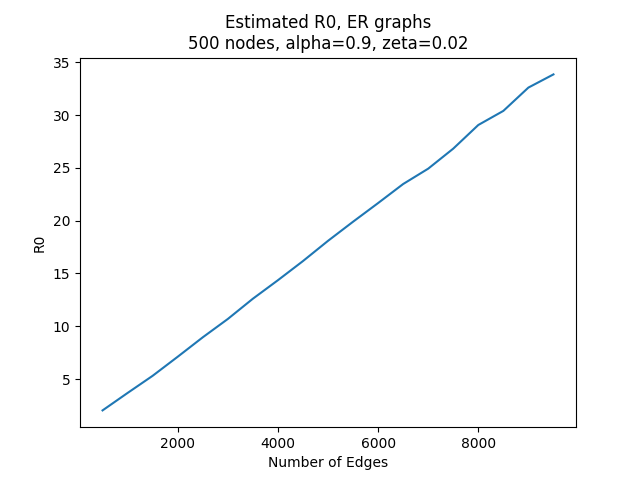
\includegraphics[scale=0.5]{images/est_r0_er.png}
    \caption{Estimated \ro values with an Erdos-Renyi contact network}
    \label{fig:r0_er}
\end{figure}

\begin{figure}[t]
    \centering
    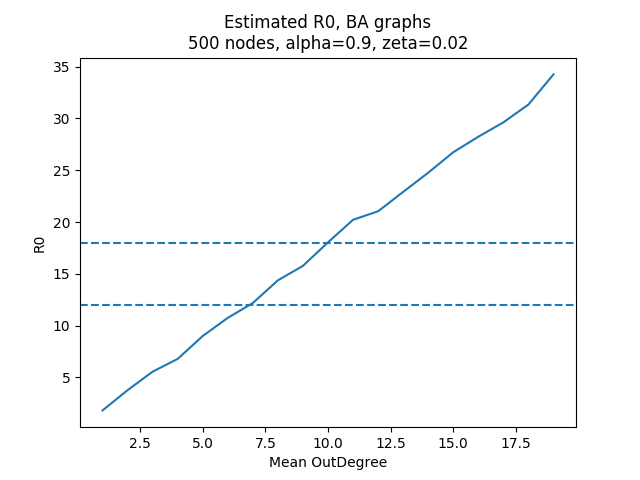
\includegraphics[scale=0.5]{images/est_ro_ba.png}
    \caption{Estimated \ro values with a Barabasi-Albert contact network}
    \label{fig:r0_ba}
\end{figure}

\begin{figure}[t]
    \centering
    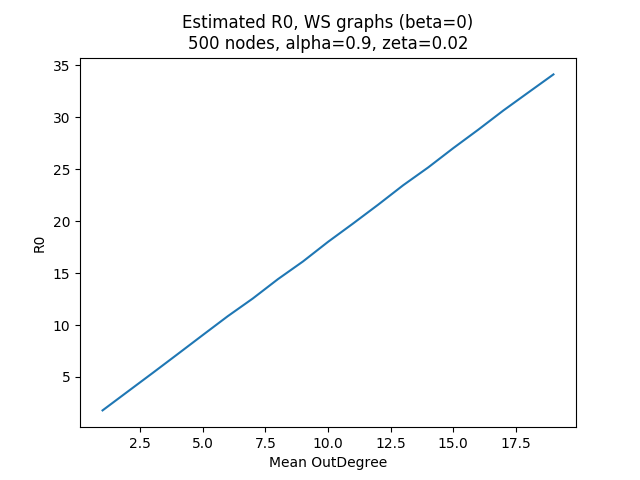
\includegraphics[scale=0.5]{images/est_r0_ws.png}
    \caption{Estimated \ro values with a Watts-Strogatz contact network}
    \label{fig:r0_ws}
\end{figure}

\begin{figure}[t]
    \centering
    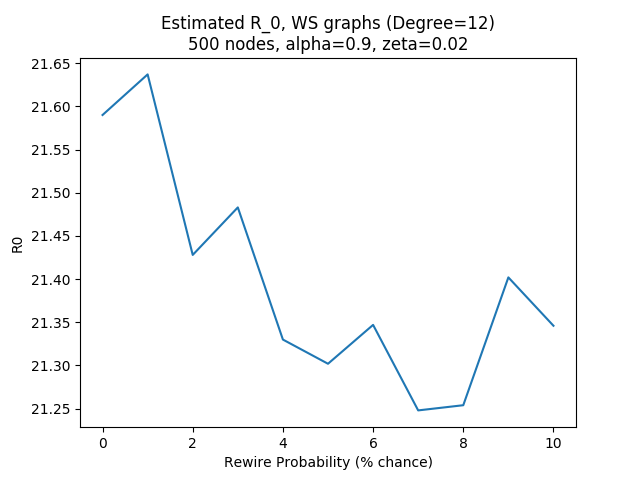
\includegraphics[scale=0.5]{images/est_r0_ws_rewire.png}
    \caption{Estimated \ro values with respect to rewiring probability parameter for Watts-Strogatz contact network}
    \label{fig:r0_ws_beta}
\end{figure}

We also evaluated our model against outbreak data taken from a case study.\cite{Mcbrein2003} We used mean squared error (MSE) to compare the predicted number of infective patients during each week with the actual number of new cases reported each week in the Dublin data. First, we tried varying the mean degree of the contact network for each of the topologies to see which topology fit the historical data the best. The outcome of these experiments is shown in figures \ref{fig:mse_er}, \ref{fig:mse_ba}, and \ref{fig:mse_ws}. From these, we determined that a lower mean degree than we had previously examined would produce the best results. We chose the Erdos-Renyi network for further optimization attempts.

\begin{figure}[t]
    \centering
    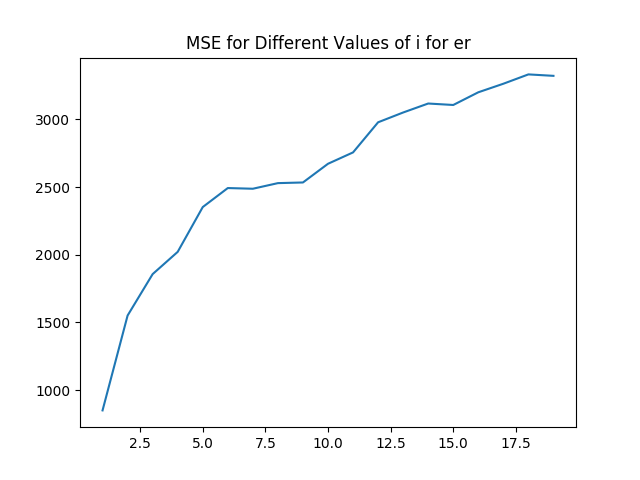
\includegraphics[scale=0.5]{images/mse_er.png}
    \caption{MSE between model and historical data, Erdos-Renyi contact network}
    \label{fig:mse_er}
\end{figure}

\begin{figure}[t]
    \centering
    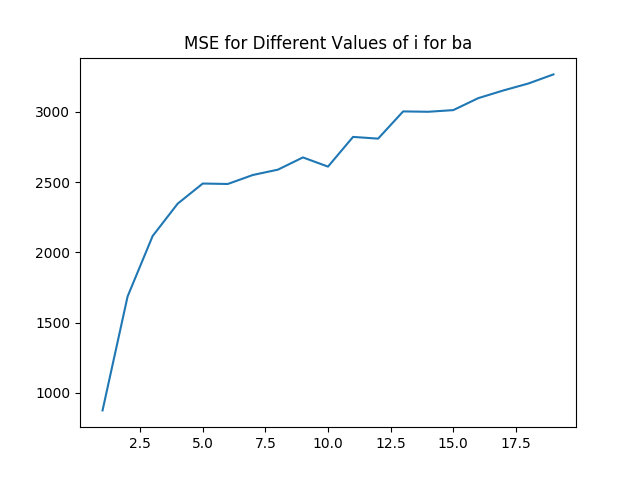
\includegraphics[scale=0.5]{images/mse_ba.png}
    \caption{MSE between model and historical data, Barabasi-Albert contact network}
    \label{fig:mse_ba}
\end{figure}

\begin{figure}[t]
    \centering
    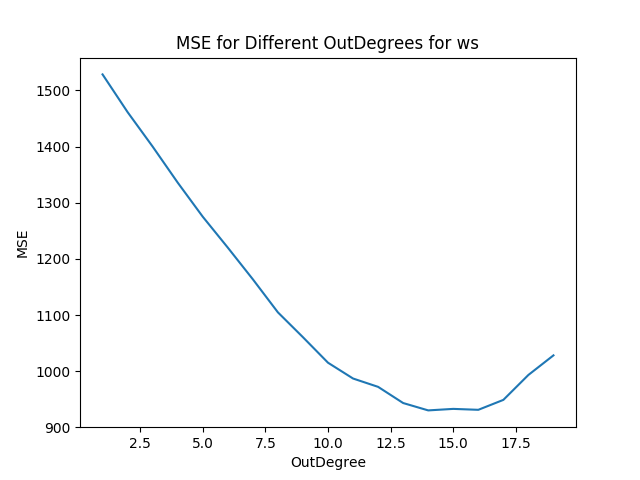
\includegraphics[scale=0.5]{images/mse_ws.png}
    \caption{MSE between model and historical data, Watts-Strogatz contact network}
    \label{fig:mse_ws}
\end{figure}

Using an ER model made it simple to generate graphs with a lower mean degree - we simply used fewer edges in the model. We again used the MSE to measure loss and varied the number of edges in the random graph model over a wide range and noted where the MSE reach a minimum. In this manner, we found that a $G(n,M)$ ER network with $n$ nodes and $n\frac{22}{20}$ edges provides the best fit between our model and the historical data with a MSE of 831.164. This is comparable to the performance of some of the models in \cite{Montalan19} Using these parameters, we ran a simulation for each 10000 different random graphs and averaged the results to produce figure \ref{fig:best_sim}.
\begin{figure}[t]
    \centering
    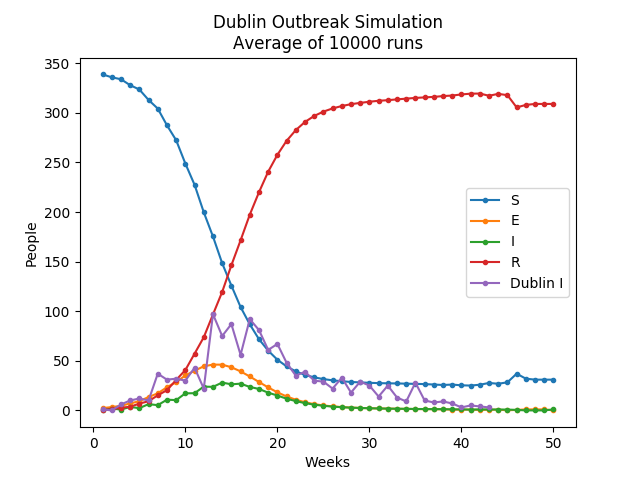
\includegraphics[scale=0.5]{images/dublin_sim.png}
    \caption{Best model predictions with historical data}
    \label{fig:best_sim}
\end{figure}

On average, there were thirty-seven people still susceptible at the end of the epidemic. This was the first example of endemic behavior we saw in our data. A contact network with more than a single connected component would prevent the infection from reaching everyone in the population. This is actually more realistic than a contact network with a single connected component because we know that measles survives despite being so virulent. If everyone in the world were in the same connected component of the contact network, measles could not survive in its current form because people become immune after infection.

The lower \ro for the real-world data could potentially be explained by immunization. A fully immune person will never become infected, so they are effectively removed from the contact graph. Under the conditions of \textit{herd immunity}, there are enough immunized people that the disease does not survive in the population. Under these conditions the contact graph is broken into many different connected components so the disease cannot propagate.\cite{pinkbookMeasles} According to the case study, immunization rates in the affected area were around 66 percent\footnote{The national average was 76\% at the time}, so a large portion of the population was not susceptible to the disease. We are ultimately interested in studying the effects of social networks on these contact networks and resulting epidemic processes. 

\section{Future Work} %Joe 
For future consideration, the authors plan to improve the time-scaling accuracy of the model to a great degree. The current model demonstrates accurate modeling for the R0 phenomena and best-fit graphs, but the time scaling is not the most accurate. For associated real-world data,\cite{Jasem2012Elsevier,Mcbrein2003,Sugarman2010} the peak of infection typically lies within the 90-120 day range due to the average incubation period of measles. In most of our simulations where R0 accuracy was given priority though, the average range was noticeably smaller than 90 days. Initially we suspected this could be due to the random graphs that we used to validate our simulations. This lead us to examine the possibility that this inaccuracy was due to the general size of the associated graphs. Increasing the population sizes made a significant difference in modeling for the WS network, but the simulated ER and BA interaction networks demonstrated similar total steps independent of the population size. As a result, different considerations will need to be made so that the model will scale well to real-world data better. Since the WS and BA networks used to validate the model are synthetic in nature, the model was not appropriately tested as rigorously against real-world estimates. Accordingly, the model will need to be properly tested against similar real-world outbreaks. So while the model preforms accurately when compared to the expected historical r0 value, improvements must be made in order to demonstrate that the model accurately generalizes when modeling all of measles' real-world behavioral facets. 


\section{Conclusion} %Seif
In this work we propose the SEIR model to describe the propagation of Measles within an interaction based network
We estimate \ro by measuring the mean degree of the contact network. We found that the lower mean degree values give the best results by using ER model to generate graphs.We consider the transition between compartments depends only on the threshold period the node should remain in that compartment.The threshold transition(TT) has a value 0 or 1. We ran the simulation for 10000 different graphs to produce the best fit figure for our SEIR model. Analysing our best fit figure we confirm that our model behave similarly to other epidemicological models and can serve to measure the propagation of the disease.

%Only includes entries that are used.
\printbibliography


\end{document}
